\subsection{الگوهای معماری زیربخش‌ها و اجزا}
\begin{RTL}
الگوهای معماری الگوهایی هستند که سطوح مختلف یک سیستم و نحوه چینش آن‌ها کنار
یکدیگر را بیان می‌کنند. این الگوها ساختار زیربخش‌ها و اجزای درشت‌دانه یک سیستم
هستند. این بخش براساس \cite{ref4} نوشته شده‌است.
\end{RTL}
\subsubsection{الگوی \lr{Layered}}
\label{archLayerSec}
\begin{RTL}
الگوی لایه‌ای \cite{ref4} دامنه‌های سیستم را بر اساس سطوح انتزاعی
مختلف به صورت سلسله‌مراتبی
سازمان‌دهی می‌کند. مفاهیم انتزاعی‌تر در یک دامنه با استفاده
از مفاهیم ملموس‌تر در دامنه‌های دیگر پیاده‌سازی می‌شوند.
این ساختار به متخصصان اجازه می‌دهد تا به طور موثر در زمینه تخصصی
خود کار کنند بدون اینکه نیاز به درک تمامی جزئیات زیرین
داشته باشند. به همین ترتیب، در توسعه نرم‌افزار،
دامنه‌های انتزاعی با استفاده از دامنه‌های ملموس‌تر پیاده‌سازی
می‌شوند که این امر موجب سازمان‌دهی و قابلیت تطبیق‌پذیری بیشتر بین
پلتفرم‌های مختلف می‌شود.
\end{RTL}
\begin{figure}[h!]
\centering
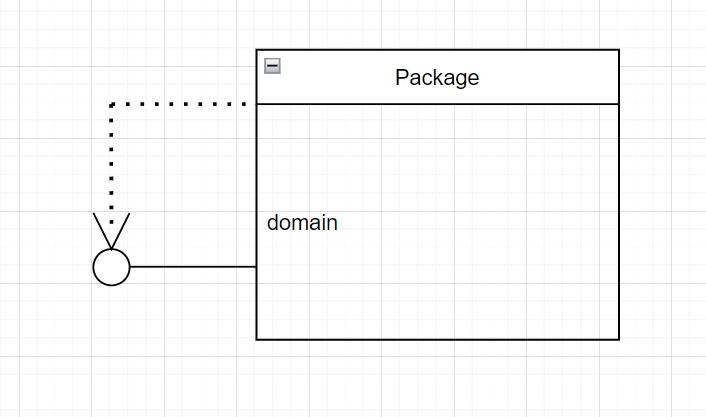
\includegraphics[scale=0.5]{images/first/layer.png}
\caption{ساختار الگوی \lr{Layered}}
\end{figure}
\subsubsection{الگوی \lr{Five Layer}}
\label{arch5LayerSec}
\begin{RTL}
الگوی معماری پنج‌لایه یک تطبیق خاص از \nameref{archLayerSec} است
که برای ساختاردهی بسیاری از سیستم‌های نهفته و بی‌درنگ
مفید است. این الگو معماری منطقی را به پنج لایه
تقسیم می‌کند که این امر به توسعه‌دهندگان کمک می‌کند
تا به راحتی ساختار سیستم‌های جدید را درک کنند.
این الگو از قابلیت انتقال بین پلتفرم‌های مختلف پشتیبانی
می‌کند و یک پلتفرم انتزاعی فراهم می‌کند که تطبیق برنامه‌ها
را آسان‌تر می‌سازد. در حالی که این الگو بسیاری از
مزایای \nameref{archLayerSec} را دارد، از جمله کارایی بالا به دلیل تعداد
کم لایه‌ها، ممکن است برای تجزیه کافی سیستم‌های پیچیده مناسب نباشد.
\end{RTL}
\subsubsection{الگوی \lr{Microkernel}}
\subsection{الگوی \lr{Channel}}
\subsubsection{الگوی \lr{Recursive Containment}}
\label{archRecContainSec}
\begin{RTL}
الگوی تجزیه و تحلیل بازگشتی برای مدیریت سیستم‌های بسیار پیچیده
با نیازمندی‌های فراوان مؤثر است. این الگو شامل شکستن سیستم به
اجزای مرتبط در سطوح مختلف جزئیات است، مانند استفاده از میکروسکوپ
با سطوح مختلف بزرگ‌نمایی. در هر سطح، اشیاء واسط‌هایی
برای همتایان خود فراهم می‌کنند و وظایف را به اجزای کوچک‌تر داخلی
تفویض می‌کنند، این تجزیه و تحلیل به صورت بازگشتی ادامه می‌یابد
تا هر بخش دارای مسئولیت ساده و متمرکز شود. این رویکرد امکان تجزیه
و تحلیل مقیاس‌پذیر را فراهم می‌کند و تأیید موارد استفاده بزرگ انتزاعی
را در هر مرحله ممکن می‌سازد و سطوح مختلفی از جزئیات رفتار سیستم را ارائه می‌دهد.
\end{RTL}
\subsubsection{الگوی \lr{Hierarchical Control}}
\label{archHierContSec}
\begin{RTL}
الگوی کنترل سلسله‌مراتبی \cite{ref4} یک
نسخه تخصصی از \nameref{archRecContainSec}
است که الگوریتم‌های پیچیده کنترلی را بین اجزای مختلف توزیع می‌کند.
این الگو از دو نوع واسط استفاده می‌کند:
واسط‌های کنترلی که نحوه دستیابی به رفتارها را نظارت و کنترل می‌کنند
و واسط‌های عملکردی که خدمات کنترل‌شده توسط واسط‌های دیگر را فراهم می‌کنند.
واسط‌های کنترلی کیفیت خدمات، مانند دقت و صحت، را تعیین می‌کنند
و سیاست‌های اجرایی را تنظیم می‌کنند. واسط‌های عملکردی رفتار مطلوب
را با استفاده از کیفیت خدمات و سیاست‌های تنظیم شده توسط واسط
کنترلی اجرا می‌کنند. این الگو با استفاده از نمودارهای حالت برای
هماهنگی اجزای زیرمجموعه و تجمیع اجزای جزء به کنترل‌کننده
از طریق ترکیب، ساختار سلسله‌مراتبی قابل تنظیم و مقیاس‌پذیری را
فراهم می‌کند. در این الگو، کنترل‌کننده وظیفه هماهنگی درخواست‌های
خدمات به عناصر جزء را دارد و اغلب از نمودارهای حالت برای نشان
دادن حالت‌های تنظیمات اجزای زیرمجموعه استفاده می‌کند. این روش
به ویژه زمانی مفید است که حالت‌های مختلف اجزای زیرمجموعه مستقل
نباشند و با استفاده از نمودارهای حالت و انطباق حالت‌ها، سازگاری میان اجزا حفظ شود.
\end{RTL}
\begin{figure}[h!]
\centering
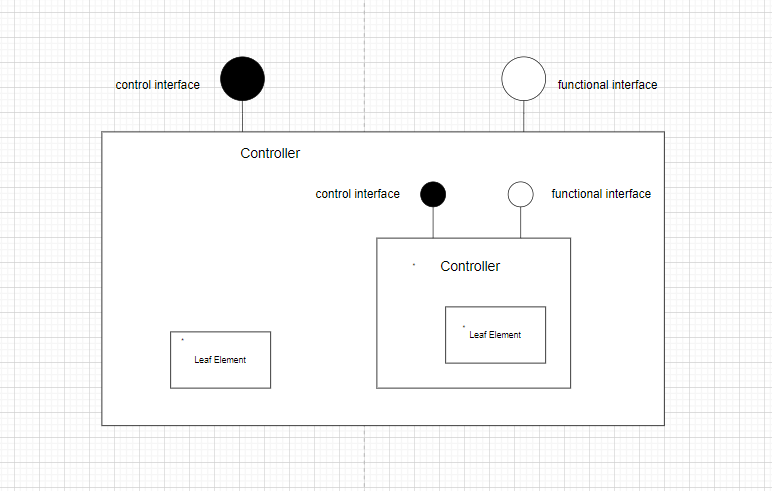
\includegraphics[scale=0.5]{images/first/hierarchical.png}
\caption{ساختار الگوی \lr{Hierarchical Control}}
\end{figure}
\subsubsection{الگوی \lr{Virtual Machine}}
\label{archVirtMachineSec}
\begin{RTL}
الگوی ماشین مجازی \cite{ref4} اولویت را
به قابلیت انتقال برنامه‌ها می‌دهد تا به کارایی
در زمان اجرا، و برای برنامه‌هایی که نیاز به اجرای روی پلتفرم‌های مختلف
دارند اما عملکرد حداکثری ضروری نیست، مناسب است.
برنامه‌ها برای یک ماشین انتزاعی نوشته می‌شوند و یک ماشین مجازی
نرم‌افزاری این دستورات را بر روی سخت‌افزار واقعی تفسیر می‌کند.
این الگو انتقال برنامه‌ها به محیط‌های جدید را ساده می‌کند،
زیرا فقط نیاز است ماشین مجازی برای پلتفرم هدف تطبیق داده شود.
اگرچه برنامه‌ها ممکن است کندتر از برنامه‌های کامپایل شده بومی اجرا
شوند، اما مزایای آن شامل ساده‌سازی انتقال و اندازه کوچکتر برنامه‌ها به
دلیل اشتراک کتابخانه‌ها در داخل ماشین مجازی است. با این حال، ماشین‌های
مجازی می‌توانند منابع زیادی مصرف کنند و ممکن است برای دستگاه‌های با
محدودیت حافظه مناسب نباشند. در چنین شرایطی ممکن است الگویی مانند
\nameref{archMicrokernelSec}
مناسب‌تر باشد.
\end{RTL}
\begin{figure}[h!]
\centering
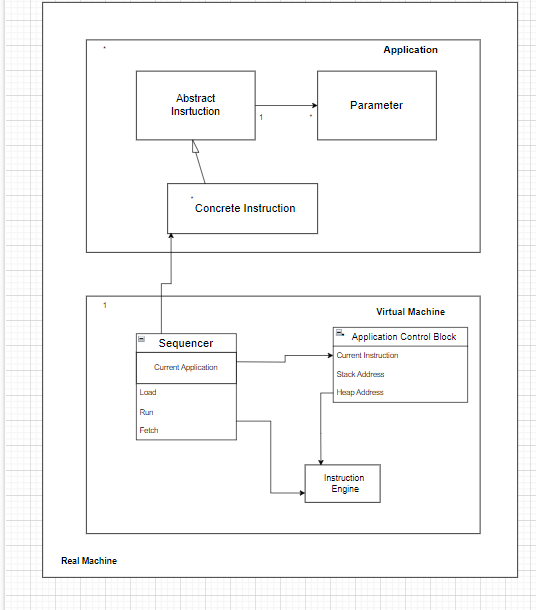
\includegraphics[scale=0.8]{images/first/virtual_machine.png}
\caption{ساختار الگوی \lr{Virtual Machine}}
\end{figure}
\subsubsection{معماری \lr{Component-Based}}
\label{archCompBasedSec}
\begin{RTL}
در \lr{UML}،
یک \lr{Component} یک اثر زمان اجرا و یک واحد قابل
جایگزینی اساسی در نرم‌افزار است
که مشابه یک شیء بزرگ‌مقیاس شامل اشیاء کوچکتری است که واسط آن را
پیاده‌سازی می‌کنند. \lr{Component}ها دارای کپسوله‌سازی قوی و
واسط‌های مستقل از زبان برنامه‌نویسی و کاملاً تعریف شده هستند.
سیستم‌های مبتنی بر \lr{Component}
که از این اشیاء بزرگ‌مقیاس به عنوان واحدهای معماری استفاده می‌کنند، از نگهداری
آسان، جداسازی عیوب، استقلال از زبان منبع، سادگی توسعه و قابلیت استفاده مجدد
بهره‌مند می‌شوند. \lr{Component}ها معمولاً اشیاء کوچکتری را
برای هدف رفتاری مشترک زمان اجرا جمع می‌کنند.
آنها دارای واسط‌های مبهم هستند، به این معنا که جزئیات
داخلی آنها از کلاینت مخفی است که این امر جایگزینی را تضمین می‌کند
اما ممکن است منجر به ناکارآمدی شود. الگوی معماری مبتنی بر مؤلفه معماری
سیستم را قوی و قابل استفاده مجدد فراهم می‌کند اما ممکن است به دلیل
استفاده از کل \lr{Component}ها حتی اگر فقط بخشی از عملکرد آنها
استفاده شود، منابع اضافی مصرف کند.
\end{RTL}
\subsubsection{الگوی \lr{ROOM}}